\begin{figure}[h!]
\centering

% Shared styles
\tikzset{
    gw cell/.style={minimum size=1.15cm, draw=black!40, thick,
                    font=\small},
    gw wall/.style={gw cell, fill=black!15},
    gw goal/.style={gw cell, fill=green!12},
    gw trap/.style={gw cell, fill=red!10},
    gw reward/.style={font=\small\bfseries},
    gw action/.style={->, thick, >=stealth, black!60,
                      shorten >=3pt, shorten <=3pt},
    gw agent/.style={circle, fill=blue!45, inner sep=4pt},
}

% Macro for the 4x3 grid skeleton
\newcommand{\gridbase}{%
    \def\s{1.15}%
    % Row 0 (bottom)
    \node[gw cell] (c00) at (0, 0) {};
    \node[gw cell] (c10) at (\s, 0) {};
    \node[gw cell] (c20) at (2*\s, 0) {};
    \node[gw cell] (c30) at (3*\s, 0) {};
    % Row 1 (middle)
    \node[gw cell] (c01) at (0, \s) {};
    \node[gw wall] (c11) at (\s, \s) {};
    \node[gw cell] (c21) at (2*\s, \s) {};
    \node[gw cell] (c31) at (3*\s, \s) {};
    % Row 2 (top)
    \node[gw cell] (c02) at (0, 2*\s) {};
    \node[gw cell] (c12) at (\s, 2*\s) {};
    \node[gw cell] (c22) at (2*\s, 2*\s) {};
    \node[gw cell] (c32) at (3*\s, 2*\s) {};
}

%% Panel (a): States -- the environment layout
\begin{subfigure}[t]{0.32\textwidth}
\centering
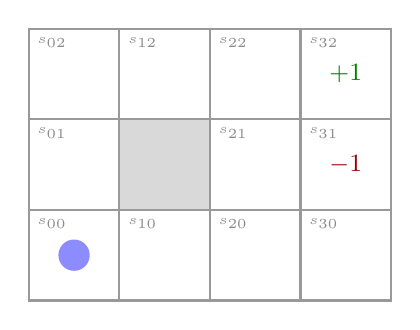
\begin{tikzpicture}
    \gridbase
    % State labels in top-left corner of each accessible cell
    \node[font=\tiny, text=black!45, anchor=north west]
          at (c00.north west) {$s_{00}$};
    \node[font=\tiny, text=black!45, anchor=north west]
          at (c10.north west) {$s_{10}$};
    \node[font=\tiny, text=black!45, anchor=north west]
          at (c20.north west) {$s_{20}$};
    \node[font=\tiny, text=black!45, anchor=north west]
          at (c30.north west) {$s_{30}$};
    \node[font=\tiny, text=black!45, anchor=north west]
          at (c01.north west) {$s_{01}$};
    % c11 is a wall -- not a state
    \node[font=\tiny, text=black!45, anchor=north west]
          at (c21.north west) {$s_{21}$};
    \node[font=\tiny, text=black!45, anchor=north west]
          at (c31.north west) {$s_{31}$};
    \node[font=\tiny, text=black!45, anchor=north west]
          at (c02.north west) {$s_{02}$};
    \node[font=\tiny, text=black!45, anchor=north west]
          at (c12.north west) {$s_{12}$};
    \node[font=\tiny, text=black!45, anchor=north west]
          at (c22.north west) {$s_{22}$};
    \node[font=\tiny, text=black!45, anchor=north west]
          at (c32.north west) {$s_{32}$};
    % Agent at start
    \node[gw agent] at (c00) {};
    % Goal and trap markers
    \node[gw reward, text=green!50!black] at (c32) {$+1$};
    \node[gw reward, text=red!60!black]   at (c31) {$-1$};
\end{tikzpicture}
\subcaption{Each cell is a \emph{state}; eleven in total.}
\label{fig:grid-world-states}
\end{subfigure}
\hfill
%% Panel (b): Actions -- movement choices
\begin{subfigure}[t]{0.32\textwidth}
\centering
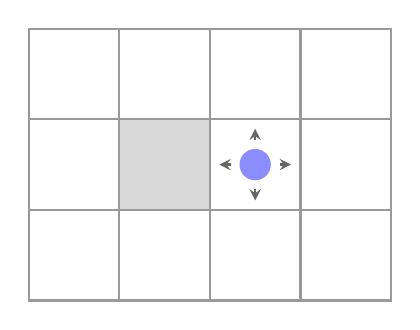
\begin{tikzpicture}
    \gridbase
    % Agent in c21 -- all four neighbors are grid cells
    \node[gw agent] (agent) at (c21) {};
    % Four action arrows to neighboring cells
    \draw[gw action] (agent.north) -- (c22.south);
    \draw[gw action] (agent.south) -- (c20.north);
    \draw[gw action] (agent.west)  -- (c11.east);
    \draw[gw action] (agent.east)  -- (c31.west);
\end{tikzpicture}
\subcaption{Moves are \emph{actions}.}
\label{fig:grid-world-actions}
\end{subfigure}
\hfill
%% Panel (c): Rewards -- feedback from the environment
\begin{subfigure}[t]{0.32\textwidth}
\centering
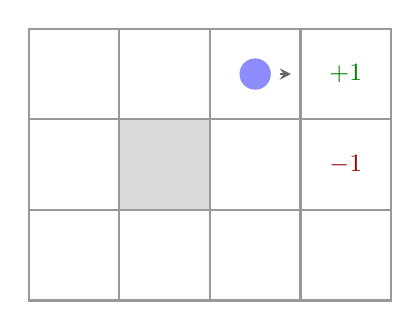
\begin{tikzpicture}
    \gridbase
    % Agent about to step into goal or trap
    \node[gw agent] (agent) at (c22) {};
    \draw[gw action] (agent.east) -- (c32.west);
    % Reward labels inside target cells
    \node[gw reward, text=green!50!black] at (c32) {$+1$};
    \node[gw reward, text=red!60!black]   at (c31) {$-1$};
\end{tikzpicture}
\subcaption{Feedback is the \emph{reward}.}
\label{fig:grid-world-rewards}
\end{subfigure}

\caption{A grid-world MDP\@. An agent (blue circle) navigates a
  $4 \times 3$ grid from a starting cell toward a goal while
  avoiding a penalty. (a)~Each accessible cell is a state, labeled
  by column and row; the shaded wall is impassable, giving eleven
  states in total. (b)~At each step the agent chooses a direction
  to move. (c)~Reaching the goal yields $+1$; the penalty
  yields~$-1$.}
\label{fig:grid-world}
\end{figure}
